\section{HMMs}
\textbf{Markov Property:} $P(X_{t+1}|X_t) = P(X_{t+1}|X_t, X_{t-1}, \dots, X_0)$\\
In words, past is independent of the future given the present.
Transitions $P(X_t|X_t-1)$ represent how state evolves over time.

\textbf{Joint Distribtion of a Markov Model:}

$P(X_0, X_1, \dots, X_T) = P(X_0) \prod_{t=1}^T P(X_t|X_{t-1})$

\textbf{Implied Conditional Independence:}
\begin{figure}[H]
    \centering
    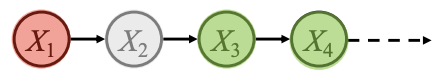
\includegraphics[width=\linewidth]{implied-cond-ind}
\end{figure}

We know that $X_3 \perp X_1 | X_2$ and $X_4 \perp X_1, X_2 | X_3$.

We also have $X_1 \perp X_3, X_4 | X_2$ by D-separation.

\textbf{Stationary Distribtion:} as $t \rightarrow \infty$, $P(X_t)$ approaches a stationary distribution $P_\infty(X)$ independent of the initial state $X_0$.
The stationary distribution encompasses all the information about the transition dynamics.

Satisfies:

$P_\infty(X) = P_{\infty + 1}(X) = \sum_x P(X|x)P_\infty(x)$

Leverage the fact that: $\sum_x P_\infty(x) = 1$.
\begin{figure}[H]
    \centering
    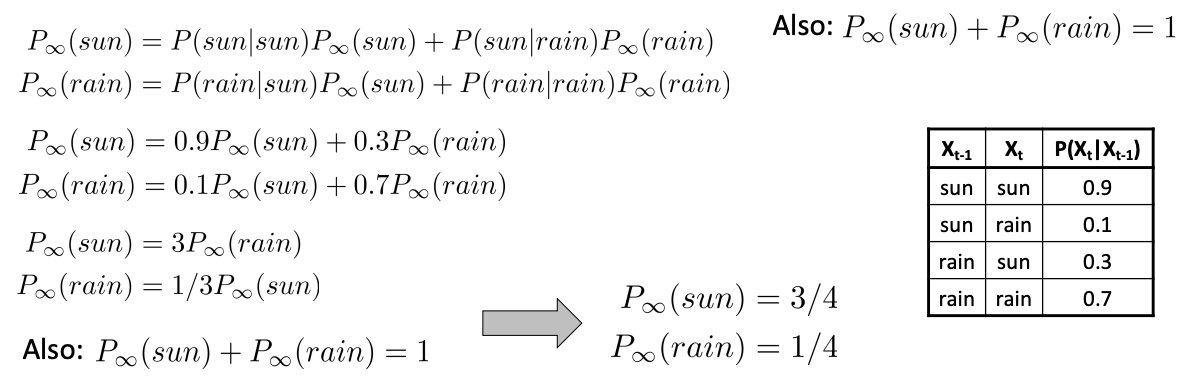
\includegraphics[width=\linewidth]{stationary-distribution}
\end{figure}

\textbf{HMMs:} Markov model with hidden states $X$ and observed states $E$.
\begin{figure}[H]
    \centering
    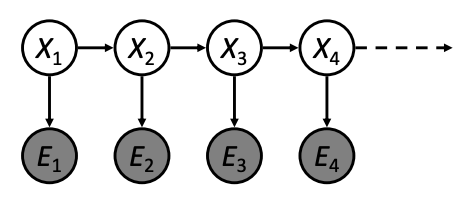
\includegraphics[width=\linewidth]{hmm}
\end{figure}

Given: $P(X_0), P(X_t|X_{t-1}), P(E_t|X_t)$

Joint Distribution = product of all CPTs since it's a BN.

Use D-separation to find conditional independence relationships.

\textbf{Update Rule:}

Let $B(s_t) = P(s_t|e_{1:t})$ and $B'(s_{t}) = P(s_{t}|e_{1:t-1})$

Elapse Time: $B'(s_{t+1}) = \sum_{s_t}B(s_t) * P(s_{t+1} | s_t) = P(s_{t+1}|e_{1:t})$

Observe Evidence: $B(s_t) \propto_{S_t} B'(s_t) * P(e_t | s_t)$

$\propto_{S_t}$ means divide the answer by the sum over all values of $S_t$: $\sum_{s_t} P(e_t, s_t | e_{1:t-1}) = P(e_t | e_{1:t-1})$.

\textbf{Worked Example:}
\begin{figure}[H]
    \centering
    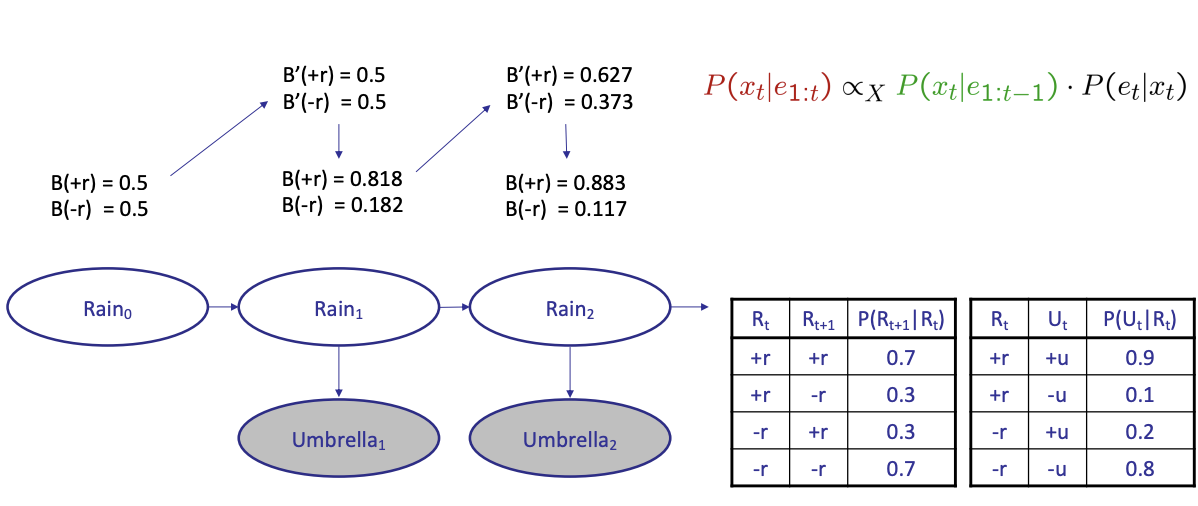
\includegraphics[width=\linewidth]{hmm-example}
\end{figure}

\textbf{Elapse Time (2nd diagonal arrow):}

$B'(+r) = B(+r) * P(+r | +r) + B(-r) * P(+r | -r) = 0.818 * 0.7 + 0.182 * 0.3 = 0.627 $

Since $R$ is a binary, $B'(-r) = 1 - B'(+r) = 0.373$

\textbf{Observe Evidence (2nd down arrow):}

New $B(+r) \propto_{R}  B'(+r) * P(+u | +r) = 0.627 * 0.9 = 0.564$

New $B(-r) \propto_{R}  B'(-r) * P(+u | -r) = 0.373 * 0.2 = 0.075 $

Normalize by sum: $0.564 + 0.075 = 0.639$:

$B(+r) = \frac{0.564}{0.639} = 0.883$

$B(-r) = \frac{0.075}{0.639} = 0.117$

